%Solución del Ejercicio 1 por medio de la metodología 6D

\subsection{Descripción del problema}
Dados 2 puntos $A \mbox{ y } B$ con coordenadas $x_{1}, y_{1}$ y $x_{2}, y_{2}$  respectivamente. Regresar la ecuación de la recta y el ángulo interno $\alpha$ que se forma entre el eje horizontal y la recta. 
%Por ejemplo con los puntos $A(2, 1)$ y $B(-3, 2)$ la ecuación debe ser $y = -\frac{1}{5}x + \frac{7}{5}$. 

\begin {figure}[h!]
\centerline{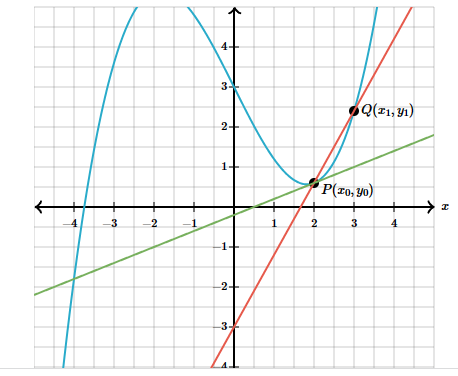
\includegraphics[width = 6cm]{Latex-imágenes/fig1 latex.png}}
\caption{Gráfica de la ecuación de la recta.}
\label{fig}
\end {figure}


\subsection{Definición del problema}
En la ecuación de la recta si dos puntos distintos $P(x_{1},y_{1})$ y $Q(x_{2},y_{2})$ se ubican en la curva $y=f(x)$ , la pendiente de la recta secante que uno los dos puntos es:

\begin{equation}
m_{sec} = \frac{y_{2} - y_{1}} {x_{2}- x_{1}} = \frac{F({x_{2}}) - {F({x_{1}})}} {x_{2}-x_{1}}
\end{equation}

Para identificar la intersección en el eje vertical se utiliza cualquiera de los 2 puntos para este caso se utilizo $P(x_{1},y_{1})$ de la siguiente forma:
\begin{equation}
    b = y_{1-} - m_{sec} * x_{1} 
\end{equation}

utilizando este método, puedes encontrar la ecuación de la recta a partir de 2 puntos dados.
y para calcular el ángulo de dicha pendiente se usa:

\begin{equation}
    \sphericalangle=\arctan(m)
\end{equation}
el algoritmo de solución implementado en el lenguaje Java empieza por la entrada de los valores $P(x_{1},y_{1})$ y $Q(x_{2},y_{2})$ solicitando sean separados por una coma.

\subsection{Diseño de la solución}
\begin {figure}[htb]
\centerline{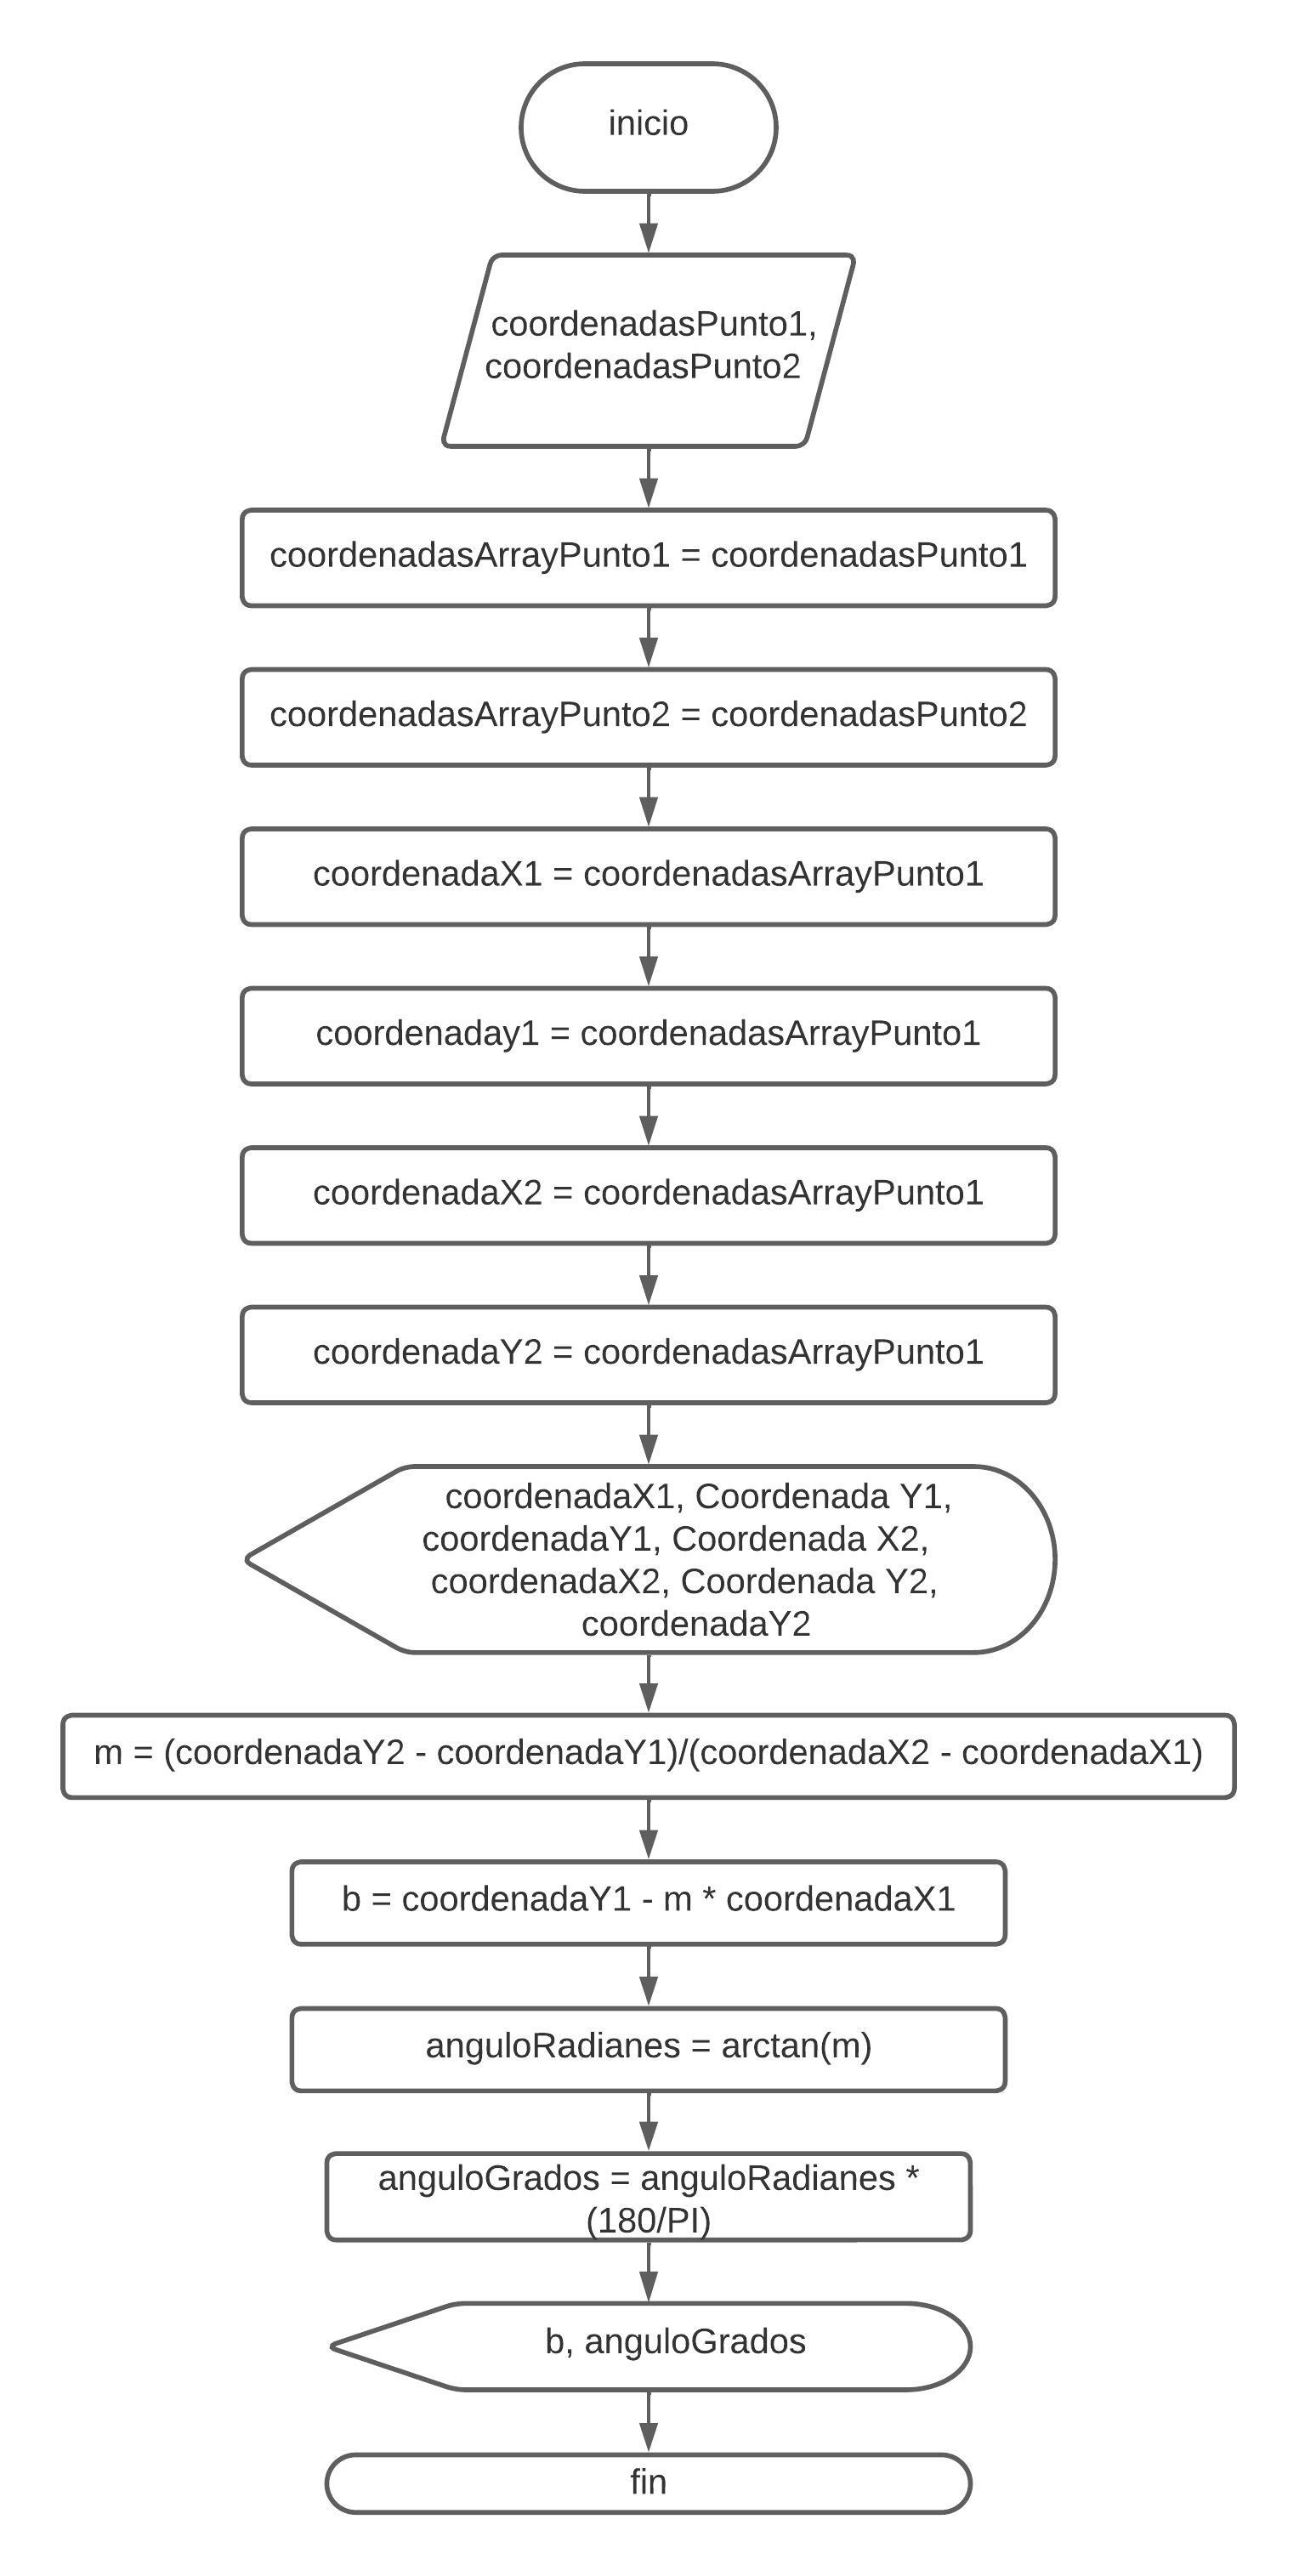
\includegraphics[width = 6cm]{Latex-imágenes/diagramaEx1.jpeg}}
\caption{Representación gráfica del algoritmo implementando la solución}
\label{fig}
\end {figure}

\subsection{Desarrollo de la solución}
Para resolver el primer problema implementamos el siguiente codigo, en el cual pide al usuario que ingrese las cordenadas el punto uno y dos separadas por una coma (,) 

\begin{javaCode}
    String coordenadasPunto1 = JOptionPane.showInputDialog("Ingrese las coordenadas del punto1(X y Y) separadas por una coma(,): ");
        
        String coordenadasPunto2 = JOptionPane.showInputDialog("Ingrese las coordenadas del punto2(X y Y) separadas por una coma(,): ");
\end{javaCode}

despues separamos los valores que el usurio ingreso, para separarlos usamos el metodo split()

\begin{javaCode}
        
        String[] coordenadasArrayPunto1 = coordenadasPunto1.split(",");
        String[] coordenadasArrayPunto2 = coordenadasPunto2.split(",");
\end{javaCode}

después con los datos ya separados los imprimimos uno por uno según los valores que ingreso el usuario, para después empezar a calcular el ángulo interno y la intersección 

\begin{javaCode}
 
        JOptionPane.showMessageDialog(null, "Coordenada X1: " + coordenadaX1 + "\n" +"Coordenada Y1: " + coordenadaY1 + "\n" + "Coordenada X2: " + coordenadaX2 + "\n" + "Coordenada Y2: " + coordenadaY2);

    double m = (coordenadaY2 - coordenadaY1)/(coordenadaX2 - coordenadaX1);
        

        double b = coordenadaY1 - m * coordenadaX1;
        
        double anguloRadianes = Math.atan(m);
        double anguloGrados = anguloRadianes * (180/Math.PI);
\end{javaCode}

y por ultimo imprimimos los resultados del ángulo interno de la recta y de la intersección 

\begin{javaCode}
     JOptionPane.showMessageDialog(null, "La intersección de la recta: " + b + "\n" + "El ángulo interno: "+anguloGrados);
\end{javaCode}

\subsection{Depuración de pruebas}

\begin{table}[h!]
  \centering
  \caption{Tabla de corridas para el Ejercicio 1.}
  \label{tab:tabla_ejemplo}
  \begin{tabular}{|c|c|c|c|c|c|}
    \hline
    \textbf{$X1$} & \textbf{$Y1$} & \textbf{$X2$} & \textbf{$Y2$} & \textbf{intersección} & \textbf{ángulo} \\
    \hline
    1 & 2 & 2 & 3 & 1 & 45\\
    2 & 4 & 6 & 8 & 2 & 0\\
    2 & 4 & 6 & 13 & 1 & 63.4349\\
    10 & 20 & 30 & 40 & 10 & 45\\
    79 & 23 & 77 & 12 & -372 & 78.6900\\
    
    \hline
  \end{tabular}
\end{table}
